\documentclass[11pt, oneside]{article}   	% use "amsart" instead of "article" for AMSLaTeX format
\usepackage{geometry}                		% See geometry.pdf to learn the layout options. There are lots.
\geometry{letterpaper}                   		% ... or a4paper or a5paper or ... 
%\geometry{landscape}                		% Activate for rotated page geometry
\usepackage[parfill]{parskip}    			% Activate to begin paragraphs with an empty line rather than an indent
\usepackage{graphicx}				% Use pdf, png, jpg, or eps§ with pdflatex; use eps in DVI mode
								% TeX will automatically convert eps --> pdf in pdflatex		
\usepackage{amssymb}
\usepackage{hyperref}
\usepackage{mathtools}
\usepackage{enumerate}
\usepackage{tikz}
\usepackage{caption}  % Required for caption outside of figure
% \usepackage[htt]{hyphenat}
\usepackage[normalem]{ulem}

\newcommand{\ck}[1]{\textcolor{cyan}{CK: #1}}
\newcommand{\jc}[1]{\textcolor{blue}{JC: #1}}


\title{Homework 1 \\ CSC 277 / 477 \\ End-to-end Deep Learning \\ Fall 2024}
\author{Henry Yin - \texttt{hyin12@u.rochester.edu}}
\date{}

\begin{document}

\maketitle

\begin{center}
    \textbf{Deadline:} 10/04/2024
\end{center}


\section*{Instructions}

Your homework solution must be typed and prepared in \LaTeX. It must be output to PDF format. To use \LaTeX, we suggest using \url{http://overleaf.com}, which is free.

Your submission must cite any references used (including articles, books, code, websites, and personal communications).  All solutions must be written in your own words, and you must program the algorithms yourself. \textbf{If you do work with others, you must list the people you worked with.} Submit your solutions as a PDF to Blackboard. 


Your programs must be written in Python. 
If a problem requires code as a deliverable, then the code should be shown as part of the solution. One easy way to do this in \LaTeX \, is to use the verbatim environment, i.e., \textbackslash begin\{verbatim\} YOUR CODE \textbackslash end\{verbatim\}.



%%%%%%%%%%%%%%%%%%%%%%%%%%%%%%%%%%%%%%%%%%%%%

\paragraph{About Homework 1:} Homework 1 aims to acquaint you with hyperparameter tuning, network fine-tuning, WandB for Training Monitoring, and model testing. \emph{Keep in mind that network training is time-consuming, so begin early!} Copy and paste this template into an editor, e.g., \url{www.overleaf.com}, and then just type the answers in. You can use a math editor to make this easier, e.g., CodeCogs Equation Editor or MathType. \href{https://blog.writefull.com/texgpt-harness-the-power-of-chatgpt-in-overleaf/}{You may use the AI (LLM) plugin for Overleaf for help you with \LaTeX formatting.}


%CodeCogs: \url{https://www.codecogs.com/latex/eqneditor.php}

%MathType: \url{http://www.dessci.com/en/products/mathtype/}
%For MathType, you have to tell it to export as LaTex. 


\clearpage

\section*{Problem 1 - WandB for Training Monitoring}

Training neural networks involves exploring different model architectures, hyperparameters, and optimization strategies. Monitoring these choices is crucial for understanding and improving model performance. Logging experiment results during training helps to:
\begin{itemize}
    \item Gain insights into model behavior (e.g., loss, accuracy, convergence patterns).
    \item Optimize hyperparameters by evaluating their impact on stability and accuracy.
    \item Detect overfitting or underfitting and make necessary adjustments.
\end{itemize}

In this problem, you'll train ResNet-18 models for image classification on the \href{https://www.kaggle.com/datasets/tanlikesmath/the-oxfordiiit-pet-dataset?select=images}{Oxford-IIIT Pet Dataset} while exploring various hyperparameters. You’ll use Weights and Biases (W\&B) to log your experiments and refine your approach based on the results.

\subsection*{Part 1: Implementing Experiment Logging with W\&B (6 points)}

\noindent \textbf{Prepare the Dataset.} Download the dataset and split it into training, validation, and test sets as defined in \texttt{oxford\_pet\_split.csv}. Complete the dataset definition in \texttt{train.py}. During preprocessing, resize the images to $224$ as required by ResNet-18, and apply \href{https://discuss.pytorch.org/t/understanding-transform-normalize/21730}{image normalization} using \href{https://stackoverflow.com/questions/73350133/how-to-calculate-mean-and-standard-deviation-of-a-set-of-images}{statistics from the training set} or from \href{https://stackoverflow.com/questions/58151507/why-pytorch-officially-use-mean-0-485-0-456-0-406-and-std-0-229-0-224-0-2}{ImageNet}.

\noindent \textbf{Evaluating Model Performance.}
During model training, the validation set is a crucial tool to prevent overfitting. Complete \texttt{evaluate()} function in \texttt{train.py} which takes a model and a dataloader as inputs and outputs the model's accuracy score and cross-entropy loss on the dataset. 

\noindent \textbf{Integrate W\&B Logging.}
To integrate W\&B for experiment logging, follow these steps and add the necessary code to \texttt{train.py}:
\begin{enumerate}
    \item Refer to the W\&B \href{https://docs.wandb.ai/tutorials/experiments}{official tutorial} for guidance.
    \item Initialize a new run at the start of the experiment following the tutorial's code snippet. Log basic experiment \textbf{configurations}, such as total training epochs, learning rate, batch size, and scheduler usage. Ensure the run \textbf{name} is interpretable and reflects these key details.
    \item During training, log the training loss and learning rate after each mini-batch.
    \item After each epoch, log the validation loss and validation accuracy.
    \item At the end of the training, log the model's performance on the test set, including loss and accuracy scores.
\end{enumerate}

\noindent \textbf{Experiment and Analysis. }
Execute the experiment using the \textbf{default} setup. Log in to the W\&B website to inspect your implementation. 

\noindent\textbf{Deliverable:}
\begin{itemize}
    \item Screenshot(s) of the experiment configuration (under the Overview tab)
    \item Screenshot(s) of all logged charts (under the Charts tab).
    \item Are the data logged accurately in the W\&B interface? Does the experiment configuration align with your expectations?
    \item Analyze the logged charts to determine whether the training has converged.
\end{itemize}


\textbf{Answer:} \\
\begin{center}
    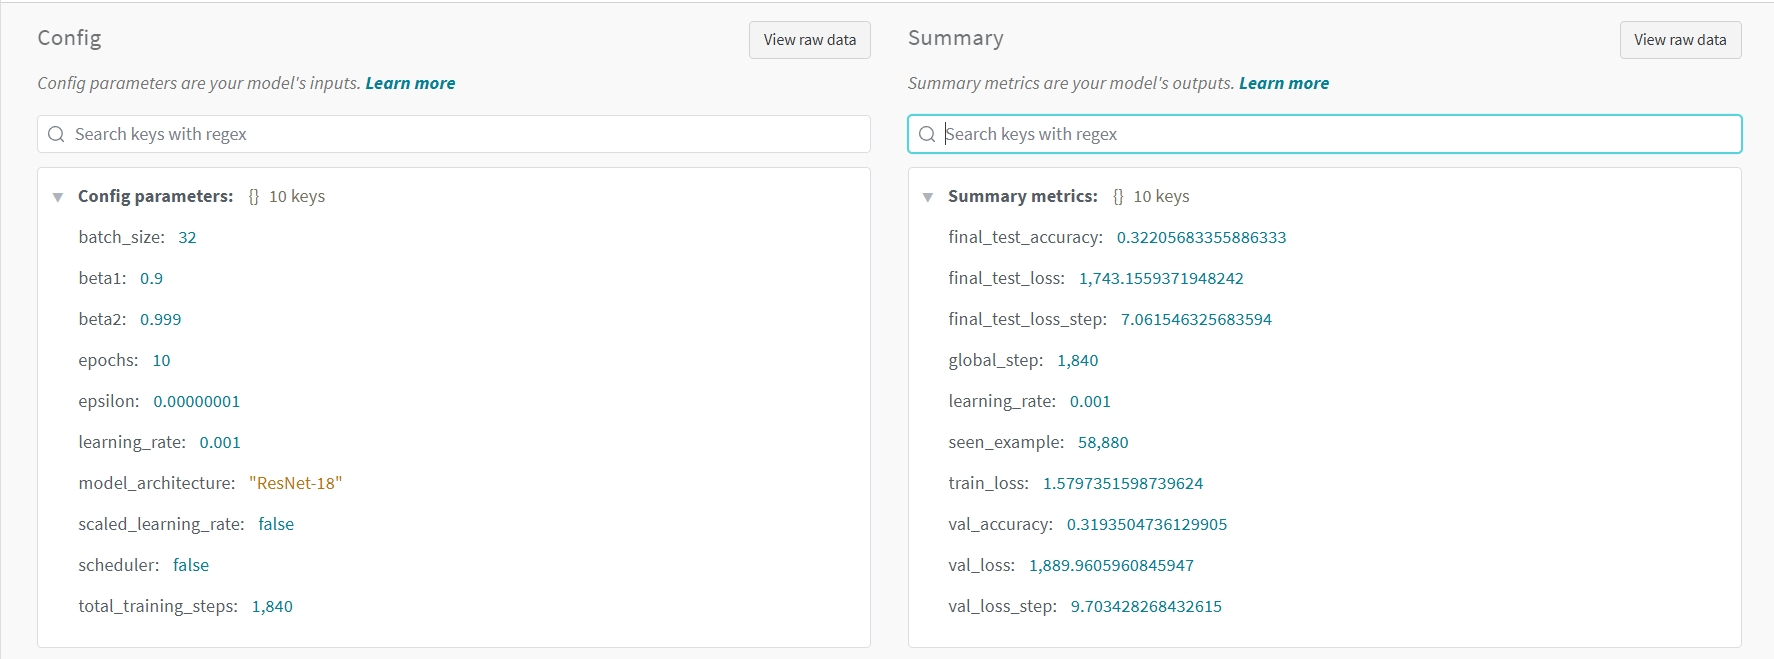
\includegraphics[width=0.5\textwidth]{p1p1_pic/Experiment_Config.png}
    \captionof{figure}{Linear Decision Boundary Graph}
\end{center}

\begin{center}
    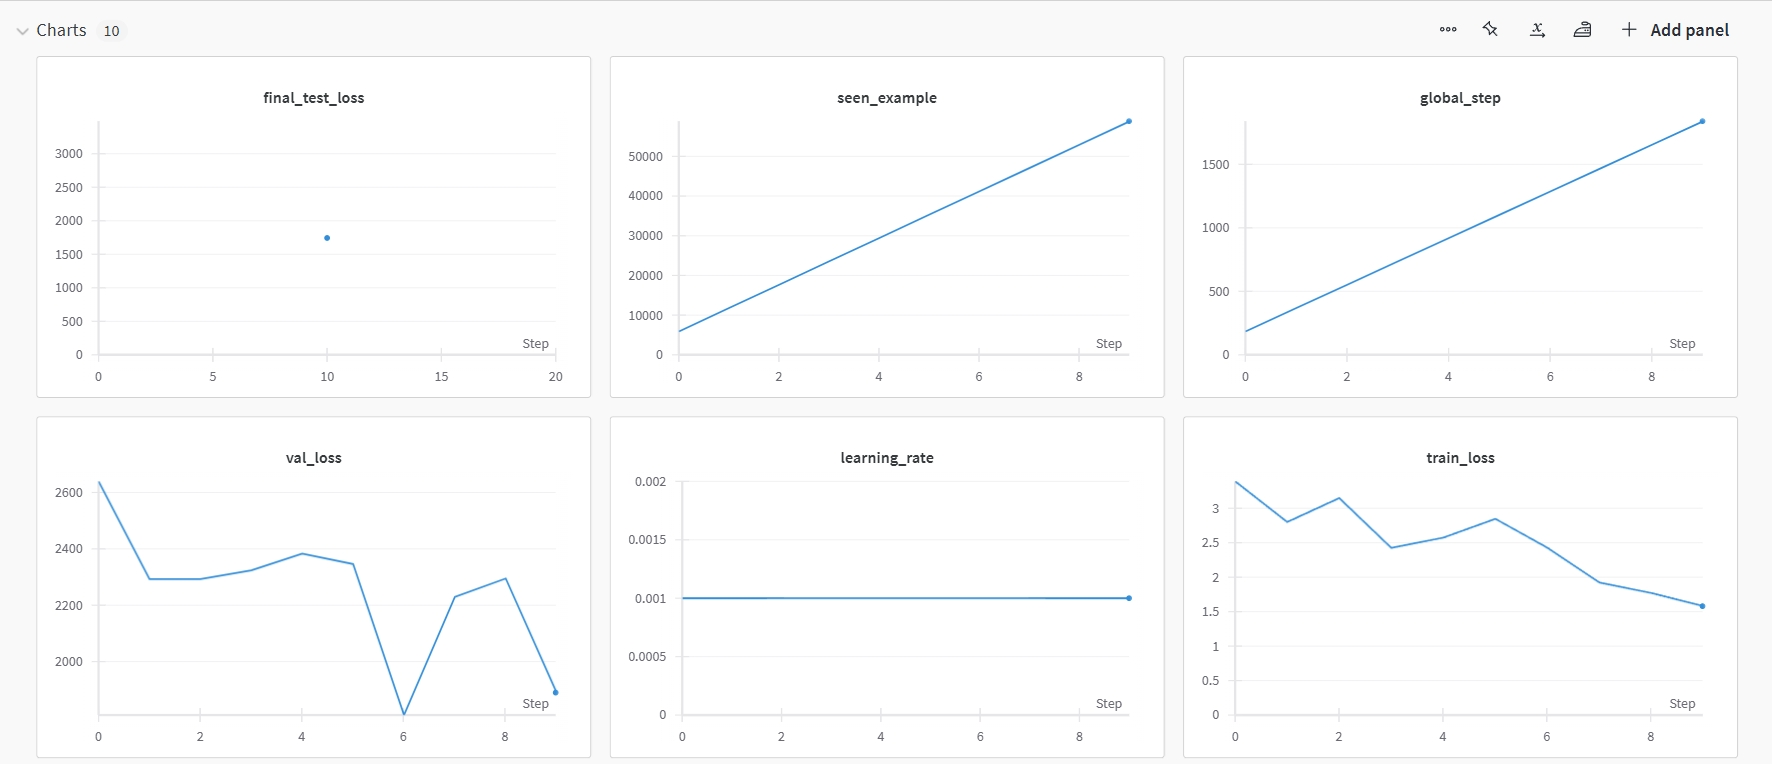
\includegraphics[width=0.5\textwidth]{p1p1_pic/Logged_Charts.png}
    \captionof{figure}{Linear Decision Boundary Graph}
\end{center}

The data has been loaded successfully to W \& B as the graph shown. 
The experiment with a realtively very low accuracy and a fluctuated loss matches my expectation since for the first sweep we have only used the default parameters on the dataset.
\\
Looking at the validation loss and validation accuracy, the former one continually grows and the latter one fluctuates hard along with epochs of training. Thus, the training is clearly not converged yet.

\subsection*{Part 2: Tuning Hyperparameters}
In this section, you'll experiment with key hyperparameters like learning rate and scheduler. For each step, change only one configuration at a time. Try not modify other hyperparameters (except batch size, which can be adjusted based on your computing resources).

\subsubsection*{2.1. Learning Rate Tuning with Sweep (5 points)}
 The learning rate is a crucial hyperparameter that significantly affects model convergence and performance.  Run the training script using \href{https://docs.wandb.ai/guides/sweeps/walkthrough}{W\&B sweep} with the following learning rates: $1e-2$, $1e-4$, and $1e-5$. Also, include the default learning rate ($1e-3$) from Part 1 in your analysis.

\noindent\textbf{Deliverable:}
\begin{itemize}
    \item Provide screenshots of logged charts showing learning rate, training loss, validation accuracy, and final test accuracy. Each chart should display results from \textbf{multiple runs} (all four learning rates in one chart). Ensure that titles and legends are clear and easy to interpret.
    \item Analyze how the learning rate impacts the training process and final performance.
    \item Code of your \href{https://docs.wandb.ai/guides/sweeps/define-sweep-configuration}{sweep configuration} that defines the search space.
\end{itemize}

\textbf{Answer:} \\
\begin{center}
    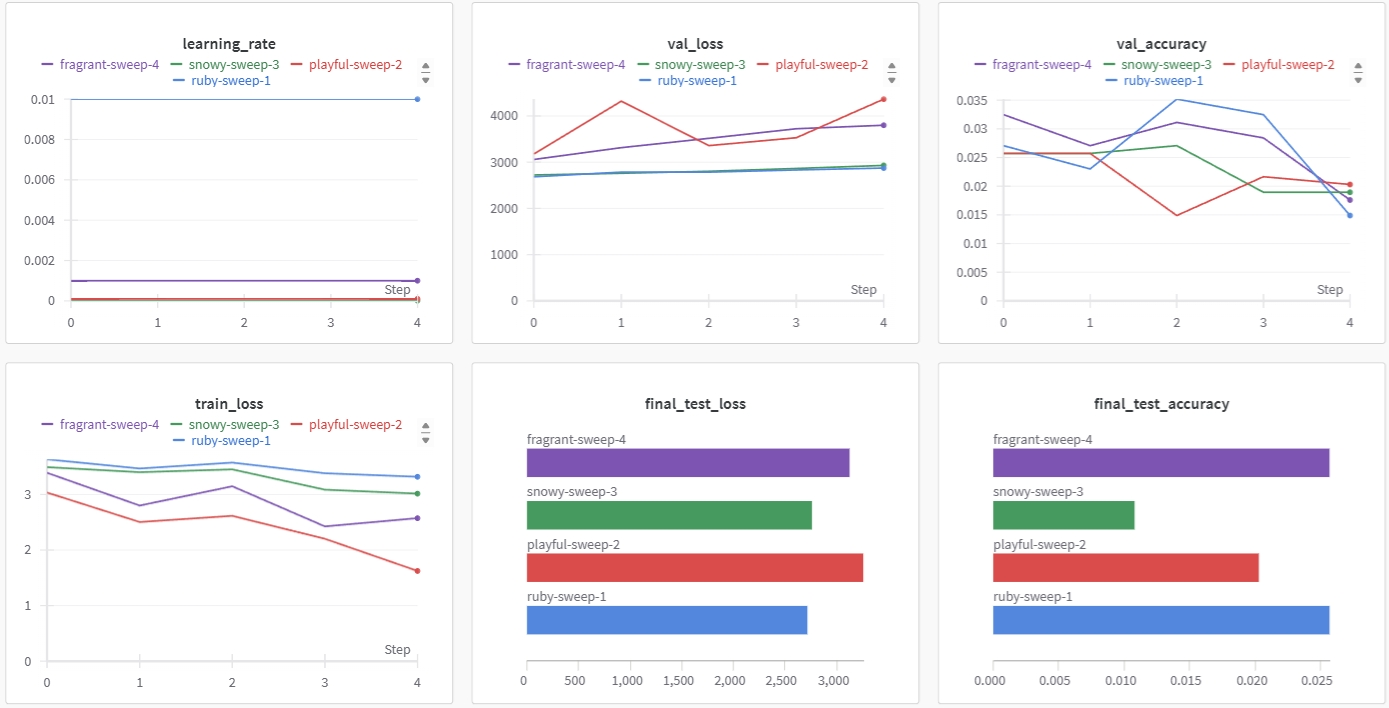
\includegraphics[width=0.5\textwidth]{p2p1_pic/SweepChart1.png}
    \captionof{figure}{Learning Rate Sweep Charts}
\end{center}

\begin{verbatim}
### Code for Sweep Config for Search Space ###
sweep_config = {
    'method': 'grid',  # Using grid method for fixed learning rates
    'metric': {
        'name': 'val_accuracy',
        'goal': 'maximize'  # Objective is to maximize validation accuracy
    },
    'parameters': {
        'learning_rate': {
            'values': [1e-2, 1e-4, 1e-5, 1e-3]  # Learning rates to test
        },
        'batch_size': {
            'values': [32]
        },
        'epochs': {
            'values': [5]
        },
        'use_scheduler': {
            # 'values': [True, False]
            'values': [False]
        }
    }
}
\end{verbatim}

\textbf{Analysis: }
\\
Lower learning rates (LR: 0.00001 and LR: 0.0001) have generally resulted in a slower reduction in training loss. This indicates that smaller steps in gradient descent might be taking more time to converge or may need more epochs to achieve lower loss. This explained why they are having realtively low final test accuracy with high final test loss.
The second highest learning rate (LR: 0.001) resulted in the fastest decrease in training loss, suggesting that realtively larger steps initially help in faster convergence for the model.

Final test loss and accuracy charts reveal that no single learning rate distinctly outperforms others across both metrics. However, the largest learning rates (LR: 0.01) tend to have lower final test loss, suggesting better generalization when large steps are used.

As a result, using the lower learning rate 0.0001 performs the best with both high accuracy and low lost for the given dataset using resnet18 network structure.

\subsubsection*{2.2. Learning Rate Scheduler (4 points)}

Learning rate schedulers dynamically adjust the learning rate during training, improving efficiency, convergence, and overall performance. In this step, you'll implement the \texttt{OneCycleLR} scheduler in the \texttt{get\_scheduler()} function within \texttt{train.py}. Compare the results to the baseline (default setting). If implemented correctly, the learning rate will initially increase and then decrease during training.

\noindent\textbf{Deliverable:}
\begin{itemize}
    \item Provide charts comparing the new setup with the baseline: learning rate, training loss, validation accuracy, and final test accuracy.
    \item Explain how the \texttt{OneCycleLR} scheduler impacts the learning rate, training process, and final performance compared to the baseline.
\end{itemize}

\textbf{Answer:} \\
\begin{center}
    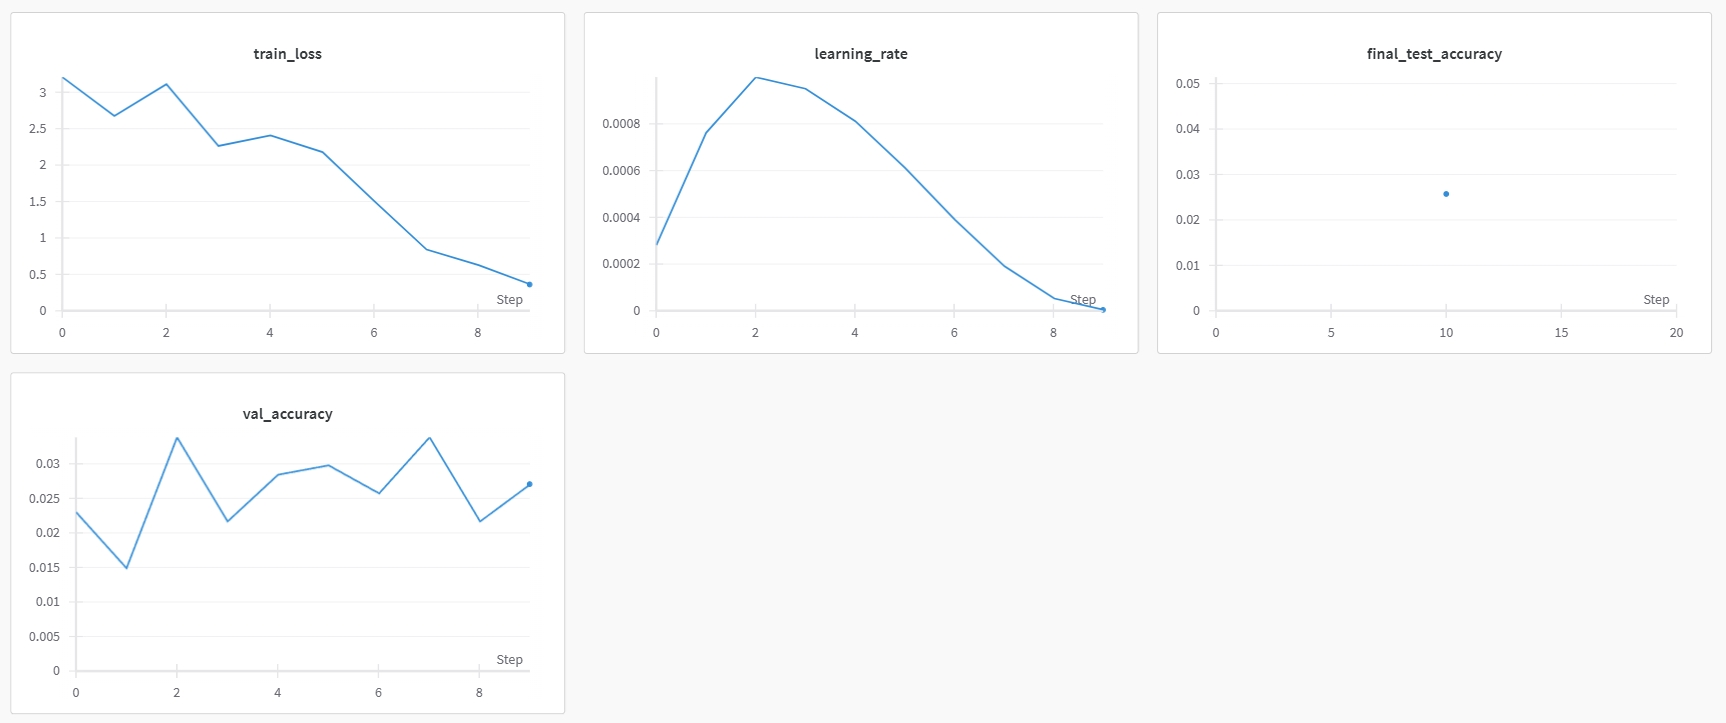
\includegraphics[width=0.5\textwidth]{p2p2_pic/SchedulerChart1.png}
    \captionof{figure}{Scheduler Chart}
\end{center}

\textbf{Analysis: }
\\
The OneCycleLR scheduler profoundly impacts the training dynamics, which is illustrated by the learning rate peaking at approximately 0.001 before sharply declining. This method accelerates initial convergence, highlighted by the training loss which quickly drops from around 3.0 to under 1.0 within the first few epochs. 
Despite such start, the validation accuracy shows considerable fluctuation, swinging between roughly 0.0339 and 0.0148, indicating a potential misalignment between training progress and generalization. 
Additionally, the final test accuracy stabilizes at about 0.02571, suggesting that while the dynamic adjustment of the learning rate helps in navigating the parameter space effectively, it might need more nuanced parameter tuning and more training epochs to fully captured the ``pattern'' of the dataset with some generalization power.

\subsection*{Part 3: Scaling Learning Rate with Batch Size (5 points)}

As observed in previous parts, the choice of learning rate is crucial for effective training. As batch size increases, the effective step size in the parameter space also increases, requiring adjustments to the learning rate. In this section, you'll investigate how to scale the learning rate appropriately when the batch size changes. Read the first few paragraphs of \href{https://www.cs.princeton.edu/~smalladi/blog/2024/01/22/SDEs-ScalingRules/}{this blog post} to understand scaling rules for Adam (used in default) and SGD optimizers. Then, conduct experiments to verify these rules. First, double (or halve) the batch size without changing the learning rate and run the training script. Next, ONLY adjust the learning rate as suggested in the post. Compare these results with the default setting. Note that since the total training steps vary with batch size, you should also log the number of seen examples to create accurate charts for comparison.

\noindent\textbf{Deliverable:}
\begin{itemize}
    \item Present charts showing: training loss and validation accuracy (with the x-axis being \texttt{seen\_examples}), and final test accuracy. Ensure the legends are clear. You may apply smoothing for better visualization. 
    \item Analyze the results: do they align with the patterns discussed in the blog post?
\end{itemize}

\textbf{Answer:} \\
\begin{center}
    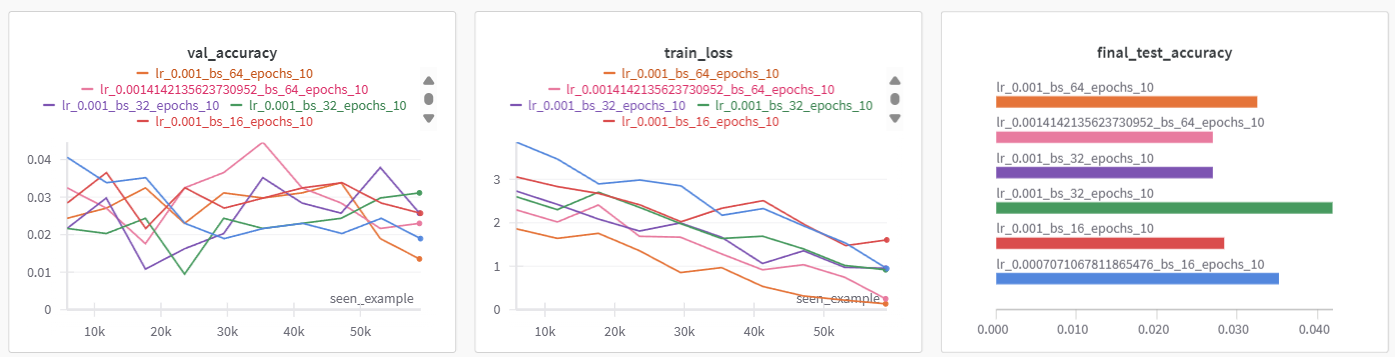
\includegraphics[width=0.5\textwidth]{p3p1_pic/ScaleLearningWBatchSizeChart1.png}
    \captionof{figure}{Scheduler Chart}
\end{center}

\textbf{Analysis: }
\\
The blog post suggests using the square root scaling rule to adjust the learning rate when changing the batch size, predicting that such adjustments should maintain or improve model performance.
\\
\begin{itemize}
    \item Validation Accuracy: The chart shows that models trained with a larger batch size ($bs\_64$) tend to have lower validation accuracy compared to models trained with a smaller batch size ($bs\_32$). This is consistent with expectation that increasing the batch size without scaling the learning rate may not improve generalization performance.
    \item Training Loss: The training loss decreases for all models, but models with smaller batch sizes (like $bs\_16$ and $bs\_32$) show a steeper decline, indicating faster convergence. The models with larger batch sizes ($bs\_64$) converge slowly, aligninh with the claim that larger batch sizes require a scaled learning rate for efficient training.
    \item Final Test Accuracy: The results show that the test accuracy is generally higher for models with smaller batch sizes ($bs\_32$), particularly when the learning rate is appropriately scaled. This indicates that increasing the batch size without scaling learning rate degrade the performance.
\end{itemize}
Overall, the results align with the blog's recommendation: scaling the learning rate appropriately when adjusting batch size helps maintain or improve model performance.

\subsection*{Part 4: Fine-Tuning a Pretrained Model (5 points)}
Fine-tuning leverages the knowledge of models trained on large datasets by adapting their weights to a new task. In this section, you will fine-tune a ResNet-18 model pre-trained on ImageNet using \texttt{torchvision.models.resnet18(pretrained=True)}. Modify the classification head to match the number of classes in your task, and replace the model definition in the original code. Keep the rest of the setup as default for comparison.


\noindent\textbf{Deliverable:}
\begin{itemize}
    \item Present charts showing: training loss, validation accuracy, and final test accuracy.
    \item Analyze the impact of pre-training on the model's learning process and performance.
\end{itemize}

\textbf{Answer:} \\
\begin{center}
    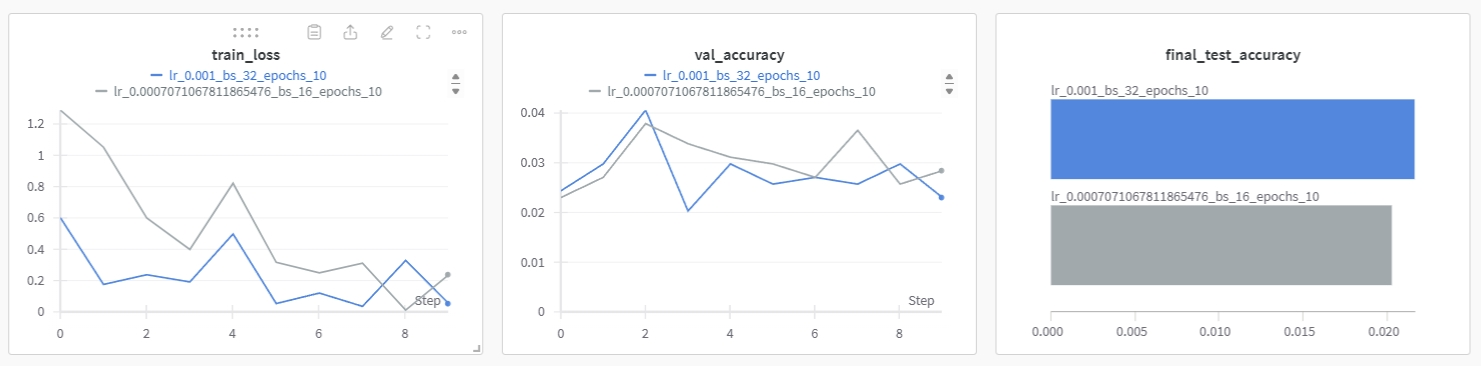
\includegraphics[width=0.5\textwidth]{p1p4_pic/PretrainModel.png}
    \captionof{figure}{Pretrained-Chart}
\end{center}
\\
Pre-training improves model initialization, accelerating convergence and enhancing performance, but the final effectiveness depends on hyperparameters like learning rate and batch size. 
In this case, model with a higher learning rate and larger batch size demonstrated faster learning and slightly better generalization, although both models showed fluctuation in validation accuracy, suggesting sensitivity to data or potential overfitting.
Fine-tuning the learning rate schedule and batch size or using data augmentation could further enhance model robustness.


\section*{Problem 2 - Model Testing}
Unlike model evaluation, which focuses on performance metrics, model testing ensures that a model behaves as expected under specific conditions:

\noindent \textbf{Pre-Train Test:} Conducted before training, these tests identify potential issues in the model's architecture, data preprocessing, or other components, preventing wasted resources on flawed training.
 \textbf{Post-Train Test:} Performed after training, these tests evaluate the model's behavior across various scenarios to ensure it generalizes well and performs as expected in real-world situations.

In this problem, you will examine the code and model left by a former employee who displayed a lack of responsibility in his work. The code can be found in the \texttt{Problem 2} folder. The necessary predefined functions for this task are available in the \texttt{model\_testing.py} file. Follow the instructions provided in that file for detailed guidance.

\subsection*{Part 1: Pre-Train Testing}

\textbf{For each question in this part, provide clear deliverables of the following:} 1. Observations and analysis of the results; 2. Suggested approaches for addressing the detected issues (if any); 3. Code implementation.

\subsubsection*{Data Leakage Check (3 points)}
Load the training, validation, and test data sets using \texttt{get\_dataset()} function. Check for potential data leakage between these sets by directly comparing the images, as data augmentation was not applied. Since identical objects usually have different hash values in Python, consider using techniques like image hashing for this comparison.

\textbf{Answer:} 
\\
\textit{Observations and analysis of the results: }
\\
The results show that there were no overlapping images found, which indicates that there is no direct data leakage from the perspective of identical images across these datasets.
\\
\textit{Suggested approaches for addressing the detected issues: }
\\
Since no data leakage was detected, there are no specific issues to address in this context but I have implemented a $remove_duplicates()$ in dataset.py function that might help resovle image overlapping.
\\
\textit{Code implementation: }
\begin{verbatim}
# Function to compute image hashes for a dataset
def compute_hashes(dataset):
    hashes = defaultdict(list)
    for idx in range(len(dataset)):
        image, _ = dataset[idx]
        # Convert tensor to PIL image for hashing
        image_pil = transforms.ToPILImage()(image)
        hash_value = imagehash.phash(image_pil)
        hashes[hash_value].append(idx)
    return hashes

# Function to find overlaps between datasets
def find_overlap(hashes1, hashes2):
    overlap = set(hashes1.keys()) & set(hashes2.keys())
    if overlap:
        print(f"Found {len(overlap)} overlapping images.")
        for h in overlap:
            print(f"Hash: {h} - Train indices: {hashes1[h]},
                 Validation/Test indices: {hashes2[h]}")
    else:
        print("No overlapping images found.")

# Function to filter out duplicates from dataset
def filter_dataset(dataset, dataset_hashes, remove_hashes):
    new_indices = []
    for h, indices in dataset_hashes.items():
        if h not in remove_hashes:
            new_indices.extend(indices)
    # Return a new subset dataset with only unique indices
    return torch.utils.data.Subset(dataset, new_indices)

# Potential duplication remove function
def remove_duplicates(train_dataset, val_dataset, test_dataset):
    # Compute hashes for each dataset
    train_hashes = compute_hashes(train_dataset)
    val_hashes = compute_hashes(val_dataset)
    test_hashes = compute_hashes(test_dataset)

    # Find duplicate hashes between train, validation, and test sets
    duplicates = {
        "train_val": set(train_hashes.keys()) & set(val_hashes.keys()),
        "train_test": set(train_hashes.keys()) & set(test_hashes.keys()),
        "val_test": set(val_hashes.keys()) & set(test_hashes.keys())
    }

    # Remove duplicates between train and validation
    train_dataset_cleaned = filter_dataset(train_dataset, train_hashes, 
        duplicates['train_val'] | duplicates['train_test'])
    val_dataset_cleaned = filter_dataset(val_dataset, val_hashes, 
        duplicates['train_val'] | duplicates['val_test'])
    test_dataset_cleaned = filter_dataset(test_dataset, test_hashes, 
        duplicates['train_test'] | duplicates['val_test'])

    print(f"Duplicates removed: Train set:
        {len(train_dataset) - len(train_dataset_cleaned)} images, "
        f"Validation set: {len(val_dataset) - len(val_dataset_cleaned)} images, "
        f"Test set: {len(test_dataset) - len(test_dataset_cleaned)} images.")

    return train_dataset_cleaned, val_dataset_cleaned, test_dataset_cleaned
\end{verbatim}

\subsubsection*{Model Architecture Check (2 points)}
Initialize the model using the \texttt{get\_model()} function. Verify that the model’s output shape matches the label format (hint: consider the number of classes in the dataset).

\textbf{Answer:} 
\begin{verbatim}
    AssertionError: Output shape mismatch: Expected (4, 10), got torch.Size([4, 128])
\end{verbatim}
\textit{Observations and analysis of the results: }
\\
model's output shape does not match the expected output shape $(batch\_size, num\_classes)$, which is $(4, 10)$, indicating that the final fully connected layer $(fc2)$ in the model is not aligned with the number of classes in the CIFAR-10 dataset.
\\
\textit{Suggested approaches for addressing the detected issues: }
\\
Removing the fc2 layer or changing it to produce num\_classes outputs directly from fc1.

\subsubsection*{Gradient Descent Validation (2 points)}
Verify that ALL the model's trainable parameters are updated after a single gradient step on a batch of data.

\textbf{Answer:}
\begin{verbatim}
    Parameter 'conv1.weight' was successfully updated.
    Parameter 'bn1.weight' was successfully updated.
    ......
    Parameter 'layer4.2.bn3.bias' was successfully updated.
    Parameter 'fc1.weight' was successfully updated.
    Parameter 'fc1.bias' was successfully updated.
\end{verbatim}
\textit{Observations and analysis of the results: }
\\
According to the code's output, by comparing the parameters after a single training step, all the learnable parameters have been updated successfully.

\subsubsection*{Learning Rate Check (2 points)}
Implement the learning rate range test using \href{https://github.com/davidtvs/pytorch-lr-finder#tweaked-version-from-fastaiauto}{pytorch-lr-finder}. Determine whether the learning rate is appropriately set by examining the loss-learning rate graph. Necessary components for \texttt{torch\_lr\_finder.LRFinder} are provided in \texttt{model\_testing.py}.

\textbf{Answer:} \\
\begin{center}
    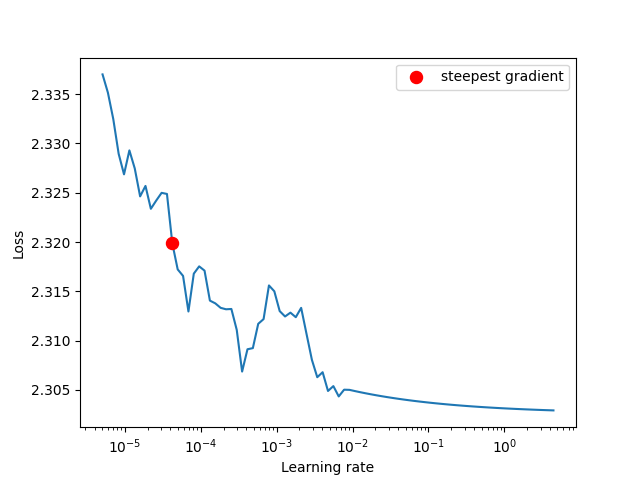
\includegraphics[width=0.5\textwidth]{p1lr_pic/learningRate.png}
    \captionof{figure}{Learning Rate Check}
\end{center}

\textit{Observations and analysis of the results: }
\\
From the learning rate range test using pytorch-lr-finder, we observe a clear pattern where the loss decreases initially as the learning rate increases. This indicates that the model is learning effectively within this range. However, after reaching a certain point (around $10^{-4}$), the loss stabilizes and eventually begins to increase, suggesting that the learning rate has surpassed the optimal point, leading to divergence. The steepest descent point identified at approximately 4.23E-05 suggests that this is the most effective learning rate for training.
\\
\textbf{All the Code implementations for above questions are avaliable in \textit{model\_testing.py} file with clear comments.}

\subsection*{Part 2: Post-Train Testing}

\subsubsection*{Dying ReLU Examination (4 points)}
In this section, you will examine the trained model for ``Dying ReLU." \href{https://datascience.stackexchange.com/questions/5706/what-is-the-dying-relu-problem-in-neural-networks}{Dying ReLU} occurs when a ReLU neuron outputs zero consistently and cannot differentiate between inputs. 
Load the trained model using \texttt{get\_trained\_model()} function, and the test set using \texttt{get\_test\_set()} function. Review the model's architecture, which is based on ResNet and can be found in \texttt{utils/trained\_models.py}. Then address the following:

\begin{enumerate}
    \item Identify the layer(s) where Dying ReLU might occur and explain why.
    \item Describe your approach for detecting Dying ReLU neurons. 
    \item Determine if Dying ReLU neurons are present in the trained model, and provide your code implementation.
\end{enumerate}
\textbf{Hint}:
Consider how BatchNorm operation would influence the presence of dying ReLU.

\textbf{Answer:} \\
Dying ReLU might occur in the deeper convolutional layers (e.g., $layer3$ and $layer4$) where the inputs might have already passed through several ReLU functions. This cumulative effect can cause more neurons to output zero, especially when weights initialized poorly or gradients vanish during backpropagation. Moreover, this issue might also occur in the initial ReLU layers ($bn1$ after $conv1$) if the preceding batch-norm (BatchNorm2d) layer scales inputs to negative values, making the ReLU output zero.
\\
To detect Dying ReLU, we can monitor outputs of all ReLU activation function during the forward pass with batch data. in detail:
\begin{itemize}
    \item Register forward ``hooks'' on each ReLU layer in the network to capture output.
    \item Counting the number of zero activations in the output tensor for each ReLU layer.
\end{itemize}
\\
\textbf{Code Implementation: }
\begin{verbatim}
def relu_hook(module, input, output):
    print(f"Hook triggered for module: {module}")
    output = output.detach().cpu()
    total_neurons = output.numel()
    dead_neurons = (output == 0).sum().item()
    activations[module] = dead_neurons / total_neurons

# Register hooks for all ReLU layers
for name, layer in trained_model.named_modules():
    if isinstance(layer, nn.ReLU):
        print(f"Registering hook for layer: {name}")
        layer.register_forward_hook(relu_hook)

# Pass a batch of data
trained_model.eval()
with torch.no_grad():
    for inputs, labels in test_loader:
        inputs = inputs.to(device)
        if inputs.dim() == 3:  # If 3D, add batch dimension
            inputs = inputs.unsqueeze(0)

        outputs = trained_model(inputs)
        break

# Display
if activations:
    for layer, percentage in activations.items():
        print(f"Layer: {layer}, Dying ReLU Percentage: {percentage:.2%}")
else:
    print("No hooks were triggered or no ReLU layers were found.")
\end{verbatim}

\subsubsection*{Model Robustness Test - Brightness (4 points)}
In this section, you will evaluate the model's robustness to changes in image brightness using a defined brightness factor.
Define a brightness factor $\lambda$, which determines the image brightness by multiplying pixel values by $\lambda$. Specifically, $\lambda = 1$ corresponds to the original image's brightness.
Load the trained model using \texttt{get\_trained\_model()} function, and the test dataset using \texttt{get\_test\_set()} function.  Investigate the model's performance across various brightness levels by adjusting $\lambda$ from $0.2$ to $1.0$ in increments of $0.2$. 

\noindent\textbf{Deliverable:}

\begin{enumerate}
    \item Plot a curve showing how model accuracy varies with brightness levels.
    \item Analyze the relationship and discuss any trends observed.
\end{enumerate}


\textbf{Answer:} 
\begin{center}
    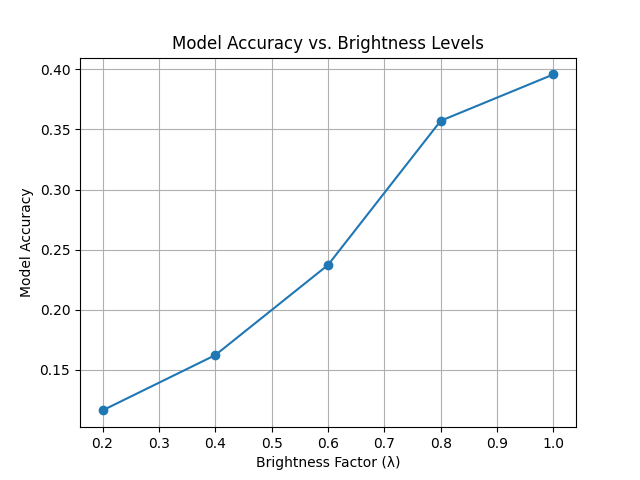
\includegraphics[width=0.5\textwidth]{p2br_pic/Brightness_accuracy.png}
    \captionof{figure}{Brightness v.s. Accuracy Chart}
\end{center}
Along with the brightness factor increases from 0.2 to 1.0, the model's accuracy steadily improves
This trend suggests that the model performs better with images that have brightness closer to original dataset's brightness level.
At lower brightness levels, the model's accuracy decreases significantly, indicating that the model is less robust to dimmer images.
Moreover, such observed patterns might potentially indicate that the model is overfitting to specific brightness conditions.

\subsubsection*{Model Robustness Test - Rotation (4 points)}

Evaluate the model's robustness to changes in image rotation. Rotate the input image from $0$ to $300$ degrees in increments of $60$ degrees. 
Similarly, load the trained model using \texttt{get\_trained\_model()} function, and the test set using \texttt{get\_test\_set()} function. 

\noindent\textbf{Deliverable:}

\begin{enumerate}
    \item Plot a curve showing the relationship between rotation angles and model accuracy.
    \item Analyze the trend and discuss any observed patterns.
    \item Suggest potential improvements to enhance model robustness
\end{enumerate}

\textbf{Answer:} \\
\begin{center}
    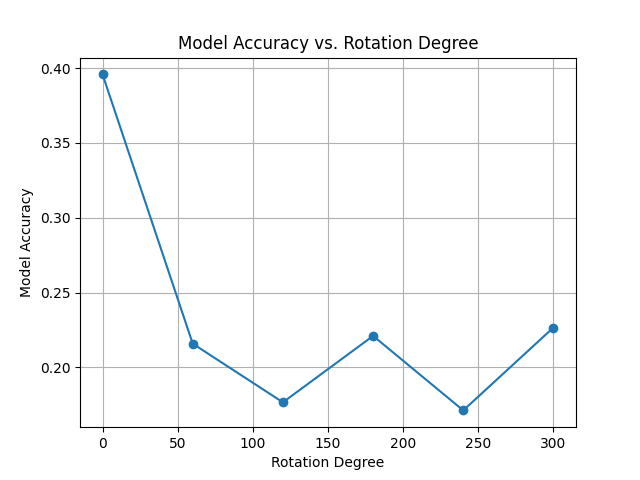
\includegraphics[width=0.5\textwidth]{p2ro_pic/Rotation_accuracy.png}
    \captionof{figure}{Rotation v.s. Accuracy Chart}
\end{center}
The graph shows that model accuracy decreases as rotation angle of input images increases from 0 to 300 degrees.
The highest accuracy is observed at 0 degrees (no rotation), and the accuracy drops sharply when the images start to rotate.
As the rotation angle increasing, the model's accuracy remains low, with  minor fluctuations. 
This tendency indicates that the model is very sensitive to rotations. 
\\
To enhance the robustness of the model, we can do:
\begin{itemize}
    \item Augment the training dataset with differnet rotations (and brightnesses) to help the model learn rotational invariance.
    \item Rotation-Invariant Architecture: Use architectures are inherently rotation-invariant, e.g., rotational convolutional layers.
    \item Fine-tuning: Fine-tune the pretrained model using datasets include a range of rotations (and brightnesses), allowing it to adapt its weights.
\end{itemize}

\subsubsection*{Normalization Mismatch (2 points)}

Load the test set using the \texttt{get\_test\_set()} function. Assume that the mean and standard deviation (std) used to normalize the testing data are different from those applied to the training data.

\noindent\textbf{Deliverable:}

\begin{enumerate} \item Calculate and report the mean and std of the images in the loaded test set (\href{https://stackoverflow.com/questions/73350133/how-to-calculate-mean-and-standard-deviation-of-a-set-of-images}{tutorial}). Compare these values with the expected mean and std after proper normalization.

\item Discuss one potential impact of this incorrect normalization on the model's performance or predictions. 

\end{enumerate}
\textbf{Answer:} \\
\begin{verbatim}
    Training Mean: [0.49139968 0.48215841 0.44653091]
    Training Std: [0.24703223 0.24348513 0.26158784]

    Testing Mean: [0.50255482 0.50009291 0.50103502]
    Testing Std: [0.28837215 0.28868326 0.28876016]

    Differences of mean in %: [2.27007456  3.71962941 12.20612156]
    Differences of std in %: [16.7346261  18.56299335 10.38745402]
\end{verbatim}
\\
The differences in both mean and standard deviation suggest that there is a mismatch in normalization between the training and testing data. The percentage difference for the standard deviation are quite significant.
This discrepancy could negatively impact the model's performance, leading to poorer generalization power.
\\
Moreover, such differences might let model receive inputs that are outside distribution of testing dataset. This can lead low accuracy, unexpected behavior, or higher error rates during testing and other potential issues.

\end{document}  